\documentclass[journal,12pt,twocolumn]{IEEEtran}

\usepackage{setspace}
\usepackage{gensymb}

\singlespacing


\usepackage[cmex10]{amsmath}

\usepackage{amsthm}

\usepackage{mathrsfs}
\usepackage{txfonts}
\usepackage{stfloats}
\usepackage{bm}
\usepackage{cite}
\usepackage{cases}
\usepackage{subfig}

\usepackage{longtable}
\usepackage{multirow}

\usepackage{enumitem}
\usepackage{mathtools}
\usepackage{steinmetz}
\usepackage{tikz}
\usepackage{circuitikz}
\usepackage{verbatim}
\usepackage{tfrupee}
\usepackage[breaklinks=true]{hyperref}
\usepackage{graphicx}
\usepackage{tkz-euclide}
\usepackage{float}

\usetikzlibrary{calc,math}
\usepackage{listings}
    \usepackage{color}                                            %%
    \usepackage{array}                                            %%
    \usepackage{longtable}                                        %%
    \usepackage{calc}                                             %%
    \usepackage{multirow}                                         %%
    \usepackage{hhline}                                           %%
    \usepackage{ifthen}                                           %%
    \usepackage{lscape}     
\usepackage{multicol}
\usepackage{chngcntr}

\DeclareMathOperator*{\Res}{Res}

\renewcommand\thesection{\arabic{section}}
\renewcommand\thesubsection{\thesection.\arabic{subsection}}
\renewcommand\thesubsubsection{\thesubsection.\arabic{subsubsection}}

\renewcommand\thesectiondis{\arabic{section}}
\renewcommand\thesubsectiondis{\thesectiondis.\arabic{subsection}}
\renewcommand\thesubsubsectiondis{\thesubsectiondis.\arabic{subsubsection}}


\hyphenation{op-tical net-works semi-conduc-tor}
\def\inputGnumericTable{}                                 %%

\lstset{
%language=C,
frame=single, 
breaklines=true,
columns=fullflexible
}
\begin{document}
\newtheorem{theorem}{Theorem}[section]
\newtheorem{problem}{Problem}
\newtheorem{proposition}{Proposition}[section]
\newtheorem{lemma}{Lemma}[section]
\newtheorem{corollary}[theorem]{Corollary}
\newtheorem{example}{Example}[section]
\newtheorem{definition}[problem]{Definition}

\newcommand{\BEQA}{\begin{eqnarray}}
\newcommand{\EEQA}{\end{eqnarray}}
\newcommand{\define}{\stackrel{\triangle}{=}}
\bibliographystyle{IEEEtran}
\providecommand{\mbf}{\mathbf}
\providecommand{\pr}[1]{\ensuremath{\Pr\left(#1\right)}}
\providecommand{\qfunc}[1]{\ensuremath{Q\left(#1\right)}}
\providecommand{\sbrak}[1]{\ensuremath{{}\left[#1\right]}}
\providecommand{\lsbrak}[1]{\ensuremath{{}\left[#1\right.}}
\providecommand{\rsbrak}[1]{\ensuremath{{}\left.#1\right]}}
\providecommand{\brak}[1]{\ensuremath{\left(#1\right)}}
\providecommand{\lbrak}[1]{\ensuremath{\left(#1\right.}}
\providecommand{\rbrak}[1]{\ensuremath{\left.#1\right)}}
\providecommand{\cbrak}[1]{\ensuremath{\left\{#1\right\}}}
\providecommand{\lcbrak}[1]{\ensuremath{\left\{#1\right.}}
\providecommand{\rcbrak}[1]{\ensuremath{\left.#1\right\}}}
\theoremstyle{remark}
\newtheorem{rem}{Remark}
\newcommand{\sgn}{\mathop{\mathrm{sgn}}}
\providecommand{\abs}[1]{\vert#1\vert}
\providecommand{\res}[1]{\Res\displaylimits_{#1}} 
\providecommand{\norm}[1]{\lVert#1\rVert}
%\providecommand{\norm}[1]{\lVert#1\rVert}
\providecommand{\mtx}[1]{\mathbf{#1}}
\providecommand{\mean}[1]{E[ #1 ]}
\providecommand{\fourier}{\overset{\mathcal{F}}{ \rightleftharpoons}}
%\providecommand{\hilbert}{\overset{\mathcal{H}}{ \rightleftharpoons}}
\providecommand{\system}{\overset{\mathcal{H}}{ \longleftrightarrow}}
	%\newcommand{\solution}[2]{\textbf{Solution:}{#1}}
\newcommand{\solution}{\noindent \textbf{Solution: }}
\newcommand{\cosec}{\,\text{cosec}\,}
\providecommand{\dec}[2]{\ensuremath{\overset{#1}{\underset{#2}{\gtrless}}}}
\newcommand{\myvec}[1]{\ensuremath{\begin{pmatrix}#1\end{pmatrix}}}
\newcommand{\mydet}[1]{\ensuremath{\begin{vmatrix}#1\end{vmatrix}}}
\numberwithin{equation}{subsection}
\makeatletter
\@addtoreset{figure}{problem}
\makeatother
\let\StandardTheFigure\thefigure
\let\vec\mathbf
\renewcommand{\thefigure}{\theproblem}
\def\putbox#1#2#3{\makebox[0in][l]{\makebox[#1][l]{}\raisebox{\baselineskip}[0in][0in]{\raisebox{#2}[0in][0in]{#3}}}}
     \def\rightbox#1{\makebox[0in][r]{#1}}
     \def\centbox#1{\makebox[0in]{#1}}
     \def\topbox#1{\raisebox{-\baselineskip}[0in][0in]{#1}}
     \def\midbox#1{\raisebox{-0.5\baselineskip}[0in][0in]{#1}}
\vspace{3cm}
\title{ASSIGNMENT 1}
\author{RONGALA ARUN SIDDARDHA :AI20BTECH11019}
\maketitle
\newpage
\bigskip
\renewcommand{\thefigure}{\theenumi}
\renewcommand{\thetable}{\theenumi}

%
Download latex-tikz code from 
%
\begin{lstlisting}
https://github.com/ArunSiddardha/EE3900/tree/main/Assignment_1/Assignment_1.tex
\end{lstlisting}
%
Download python code from 
%
\begin{lstlisting}
https://github.com/ArunSiddardha/EE3900/tree/main/Assignment_1/code/Assignment_1.py
\end{lstlisting}
\section{PROBLEM}
If the vertices of an isoceles triangle are given by  $\vec{B} = \myvec{-2\\-2}$, $\vec{A}=\myvec{-1\\2}$ and $\vec{C}=\myvec{3\\1}$ .Find the distance of the vertex A from the base of the triangle 
\section*{SOLUTION}
Since, Given that triangle is iscoceles let us check which two sides are equal,
\begin{align*}
    BC = a = \norm{\vec{B} - \vec{C}} &= \sqrt{(-2-3)^{2}+ (-2-1)^{2}}\\
    &= \sqrt{25 + 9}\\
    &= \sqrt{31}\\
    AB = c = \norm{\vec{A} - \vec{B}} &= \sqrt{(-1+2)^{2}+ (2-(-2))^{2}}\\
    &= \sqrt{1 + 16}\\
    &= \sqrt{17}\\
    CA = b = \norm{\vec{C} - \vec{A}} &= \sqrt{(3+1)^{2}+ (1-2)^{2}}\\
    &= \sqrt{16 + 1}\\
    &= \sqrt{17}
\end{align*}
So, we can see that sides AB , AC are same.\\
So, the distance between A and the side BC is same as distance between the vertex A and mid point D the side BC.\\\\
Mid point of BC is
\begin{align*}
     \vec{D}= \frac{\vec{B} + \vec{C}}{2} = \myvec{\frac{3-2}{2}\\\frac{1-2}{2}}=\myvec{\frac{-1}{2}\\ \frac{-1}{2}}
\end{align*}
\begin{figure}[htp]
    \centering
    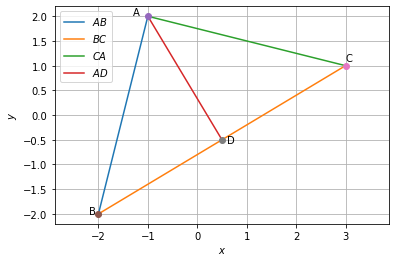
\includegraphics[width=\columnwidth]{Assignment_1.png}
    \caption{plot}
    \label{fig:my_label}
\end{figure}
\begin{align*}
    AD = \norm{\vec{A} - \vec{D}} &= \sqrt{(-1-\frac{1}{2})^{2} + (2-\frac{-1}{2})^{2}}\\
    &= \sqrt{\frac{9}{4} + \frac{25}{4}}\\
    &= \sqrt{\frac{34}{4}}\\
    &= \frac{\sqrt{34}}{2}
\end{align*}
Therefore the distance is $\frac{\sqrt{34}}{2}$
\end{document}
